\documentclass[french, a4paper, francais, frenchb, fr, 12pt]{report}


\usepackage[utf8]{inputenc}
\usepackage[T1]{fontenc}
\usepackage{graphicx}

\usepackage{titling}
\newcommand{\subtitle}[1]{
  \posttitle{
    \par\end{center}
    \begin{center}\large#1\end{center}
    \vskip0.5em}
}



\begin{document}


\chapter*{Remerciement}
\begin{center}
\Large \textbf{\textit{Tout d'abord, nous remercions Allah, notre créateur, pour nous avoir donné la force, la volonté et le courage d'accomplir ce modeste travail.\\
Nous remercions notre encadreur Monsieur Allaoui ansi que Madame Kerrouche pour leurs conseils et leur encouragement du début jusqu'à la fin de ce travail.\\
Nos remerciements vont aussi à tous ceux qui ont contribué de près ou de loin à la réalisation de ce travail.\\Enfin, nous tenons à exprimer notre profonde gratitude à nos familles qui nous ont toujours soutenus et à tous ceux qui ont participé à la réalisation de ce mémoire. Ainsi qu'à tous les enseignants qui ont contribué à notre formation.}}
\end{center}

\chapter*{Dédicaces}
\begin{center}
\Large \textbf{\textit{Nous dédions ce modeste travail à nos parents bien-aimés qui nous ont soutenus tout au long de notre cursus universitaire et le sont toujours.\\
À nos amis qui n'ont jamais hésité à nous aider de quelque manière que ce soit.\\
Et à tous ceux qui nous ont enseigné tout au long de notre vie scolaire.\\
A nos camarades de la 3ème année LMD.\\
Merci à tous.}}
\end{center}

\newpage
\begin{abstract}
this is the abstract
\end{abstract}


\tableofcontents

\newpage
\listoffigures

\newpage
\listoftables


\newpage
\chapter*{Liste des Abréviations}
\addcontentsline{toc}{chapter}{Liste des Abréviations}
	\begin{itemize}
		\item \textbf{MVC}:  Model View Controller
		\item \textbf{UI}: User Interface
		\item \textbf{SDK}: Software Development Kit
		\item \textbf{UML}: Unified Modeling Language
		\item \textbf{NoSQL}: Not only Structured Query Language
		\item \textbf{JSON}:  Java Script Object Notation
	\end{itemize}


\newpage
\chapter*{Introduction}
    Au cours de la dernière décennie, nous avons assisté à une révolution dans les commerces en ligne. Les gens se sont habitués aux achats en ligne et aux réservations à distance comme la réservation de billets, l'achat d'articles et même la commande de nourriture, principalement parce que c'est plus rapide, sans effort et moins compliqué.

Lorsque quelqu'un veut acheter des repas en ligne, il doit chercher un restaurant qui prépare les repas désirés. La commande doit lui être livrée soit par le livreur du restaurant, soit par un établissement de livraison séparé.

Dans les pays étrangers, en Europe ou aux États-Unis, beaucoup de restaurants et de sociétés de livraison ont leur propre application mobile. Malheureusement, ce n'est pas le cas pour tous les établissements qui peuvent se permettre de créer leur propre application en raison des coûts élevés de développement d'une application mobile.

Delàs, nous avons pensé à contribuer à une solution. C'est une plateforme conçue comme une application mobile qui regroupe les clients, les restaurants et les établissements de livraison en un seul endroit. \\Elle répond à tous les besoins des personnes qui veulent commander leurs plats à distance, elle permettra également aux propriétaires de restaurants et aux établissements de livraison d'augmenter leurs ventes et d'accélérer leur flux de travail avec les clients à distance.

\addcontentsline{toc}{chapter}{Introduction}

\newpage
\chapter{Receuil des besoins} Dans cette partie, nous proposons de regrouper les besoins techniques necessaires pour accomplir ce travail.
	\section{Développement Android} Nous avons choisi de réaliser une application mobile dédiée aux utilisateurs d'Android. Il existe beaucoup de choix quant aux technologies que nous allons utiliser pour ce développement.
		\subsection{Les technologies utilisées} Dans ce travail nous avons utilisé le framework Flutter pour les interfaces et la logique de l'application et Cloud Firestore de Firebase pour le stockage et la gestion de la base de données.
			\subsubsection*{Flutter} C'est un SDK d'interface utilisateur open-source créé par Google. Il est utilisé pour développer des applications multiplateformes pour Android, iOS, Linux, Mac, Windows et le Web à partir d'une base de code unique.\\Nous avons utilisé Flutter en raison de sa structure qui favorise la vitesse de développement. Sa structure est simplement une cascade de widgets faciles à personnaliser.

Flutter utilise le langage de programmation Dart, également développé par Google. Il s'agit d'un langage orienté objet, basé sur des classes avec une syntaxe de type de la language C.
			\subsubsection*{Firebase} C'est une plateforme accessible de n'importe quel endroit, qui aide à développer rapidement des applications de qualité. Elle dispose de nombreuses fonctionnalités, mais nous l'utilisons principalement pour son service de stockage au Cloud (Cloud Firestore).\\
				\paragraph*{Cloud Firestore} est une base de données documentaire NoSQL (un ensemble de continuation en cascade collection-document) qui nous permet de stocker, de synchroniser et d'interroger facilement des données pour des applications mobiles et web à l'échelle mondiale.
	\section{Méthode de travail collaborative}
		L'application conçue dans ce travail, a été développée à partir de zéro par trois développeurs. Nous avons travailler en parallèle sur le même projet, de ce fait nous, les trois développeurs, allons donc utiliser Git et Github.

		\subsection*{Git} C'est un logiciel permettant de suivre les modifications apportées à un ensemble de fichiers. Il est généralement utilisé pour coordonner le travail des programmeurs qui collaborent à l'élaboration du code source lors du développement de logiciels. Ses objectifs sont la rapidité, l'intégrité des données et la prise en charge des flux de travail distribués et non linéaires.

		\subsection*{Github} C'est un service d'hébergement de référentiel Git, mais il ajoute de nombreuses fonctionnalités qui lui sont propres. Il fournit une interface graphique basée sur le Web. Il fournit également un contrôle d'accès et plusieurs fonctions de collaboration.
	\section{Architecture du code} %include the sequence chart of flutter in mvc
		Nous avons utilisé l'architecture de projet MVC. Il s'agit d'un modèle de conception de logiciel couramment utilisé pour développer des interfaces utilisateur qui divisent la logique du programme en trois éléments interconnectés.

Cela permet de séparer les représentations internes de l'information de la manière dont l'information est présentée à l'utilisateur et acceptée par celui-ci.
\begin{figure}[!h]
  \center
  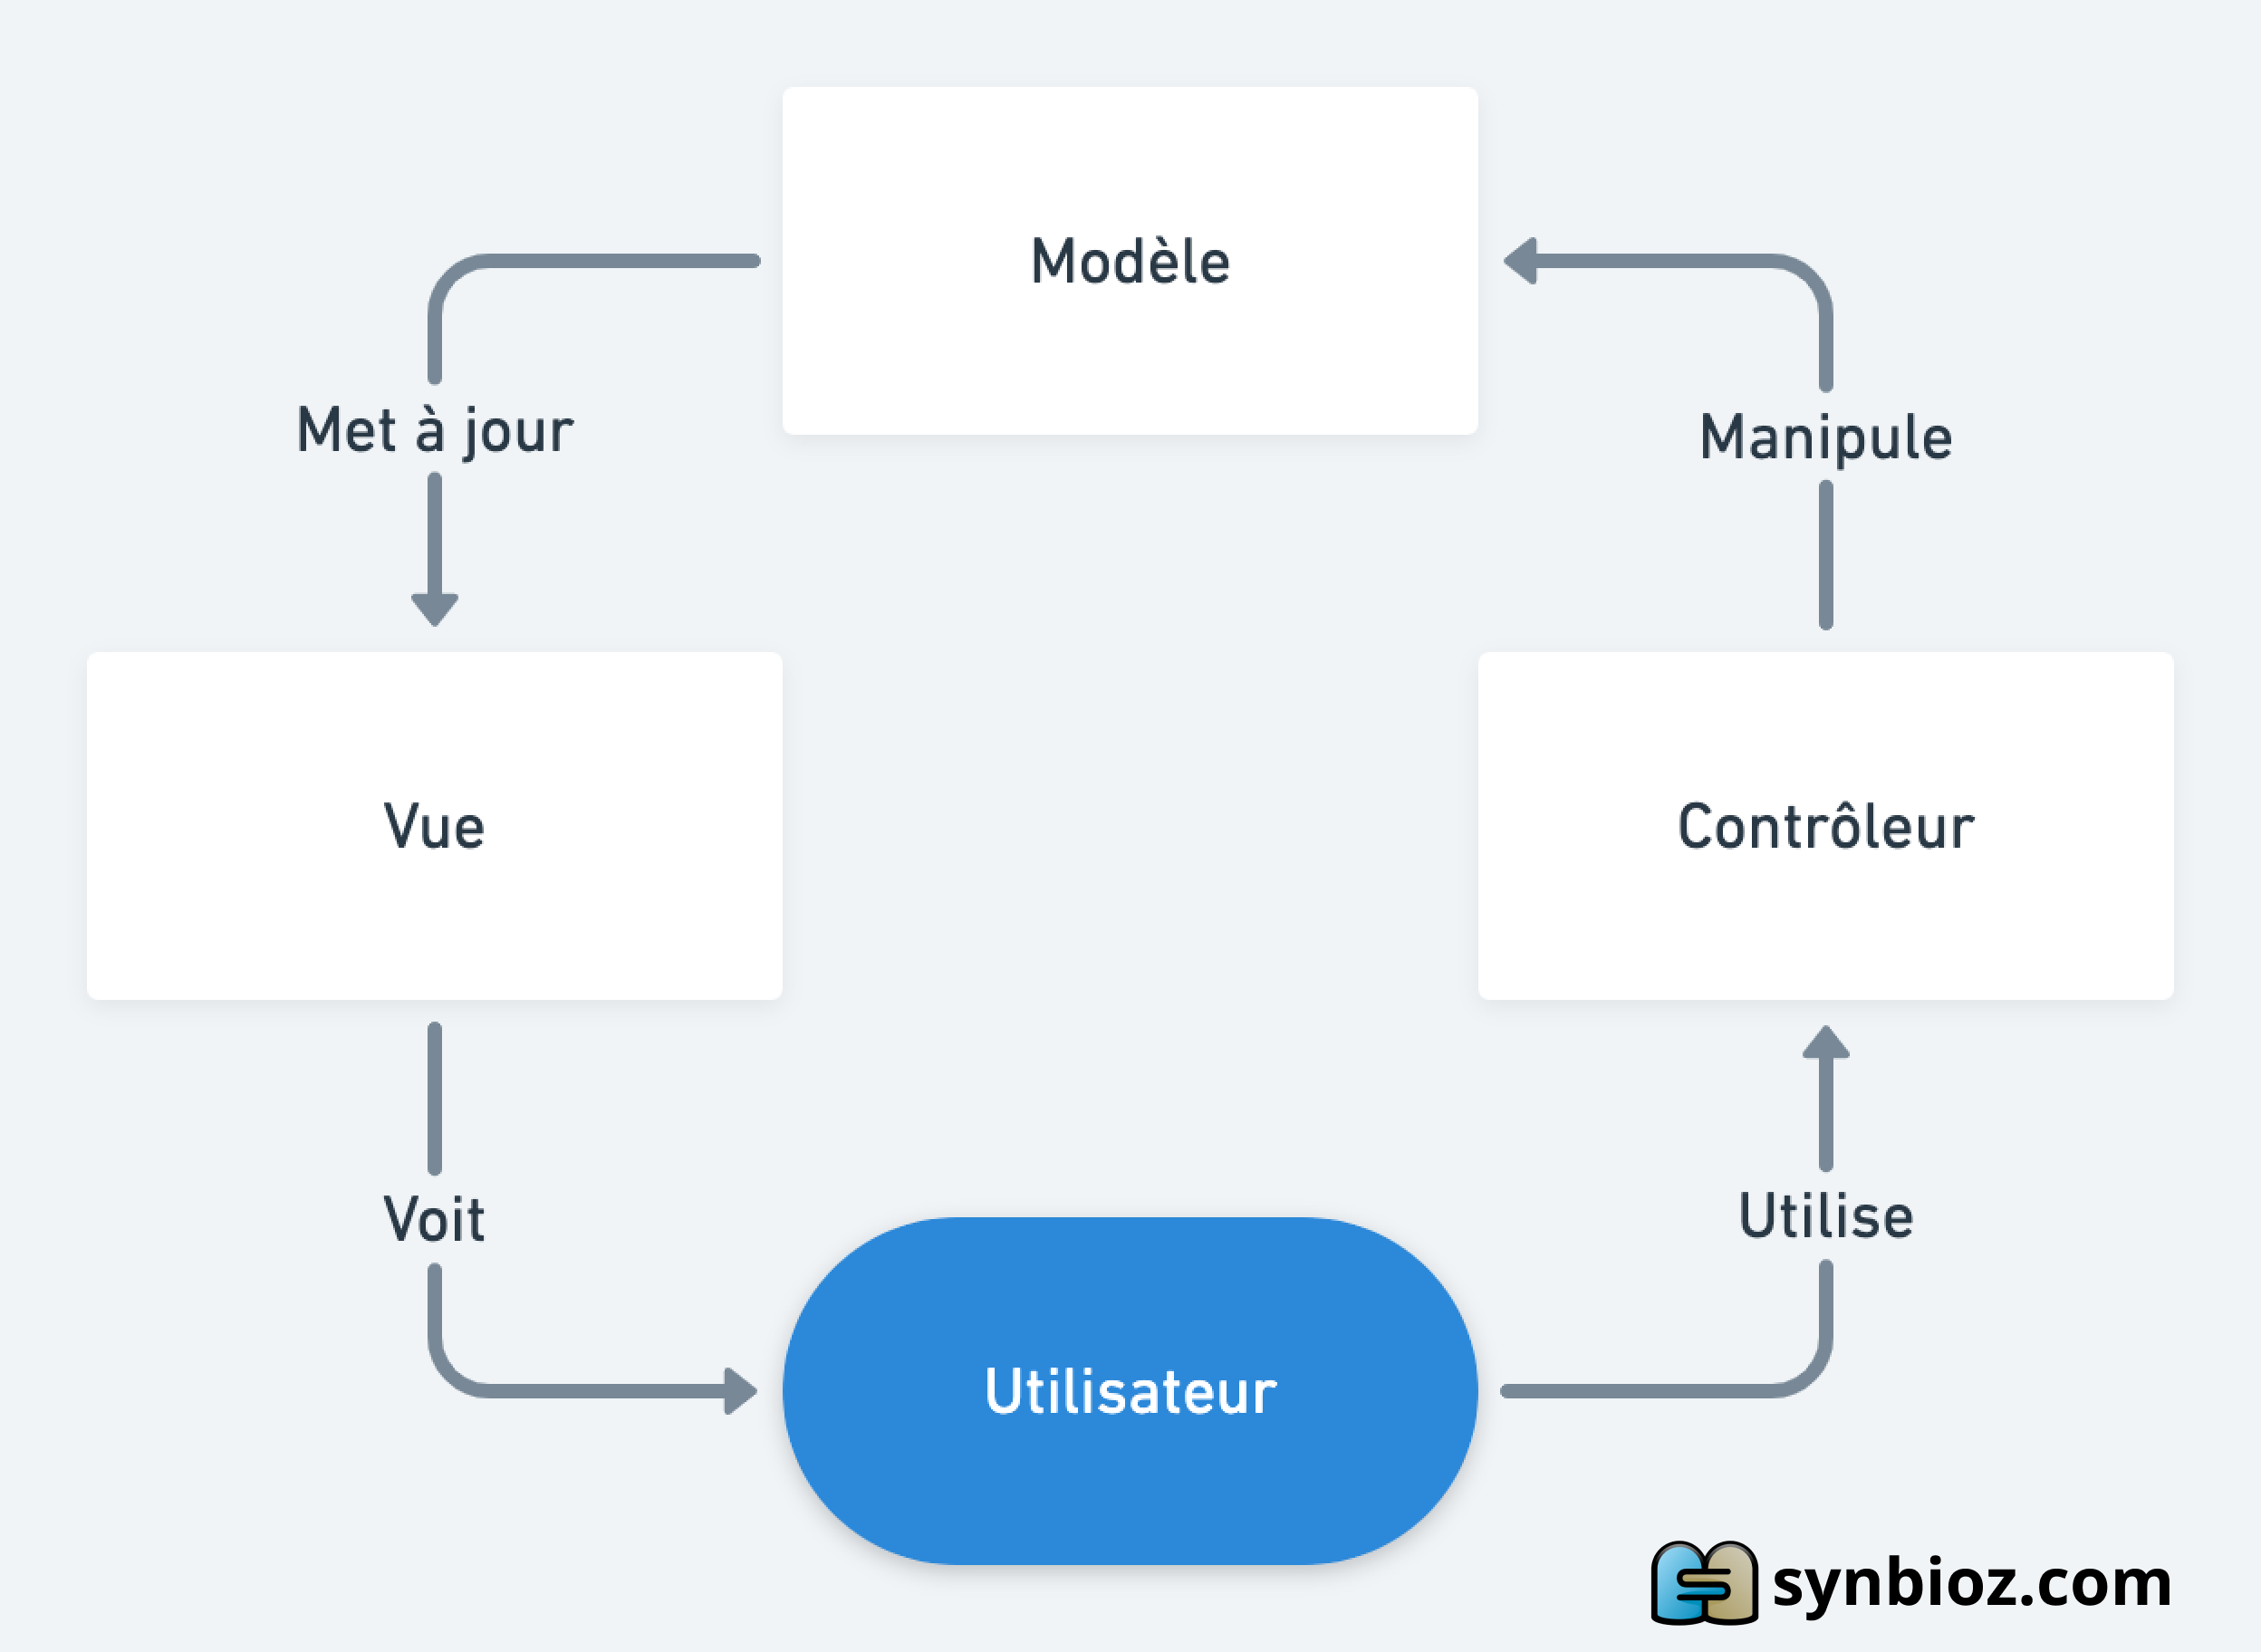
\includegraphics[width=10cm]{mvc.png}
  \caption{Le flux MVC}
  \label{fig:fluxmvc}
\end{figure}

\newpage
\chapter{Conception de l'application} Dans ce chapitre nous présentons les differentes étapes de la conception de l'application de gestion de commande et livraison de la restauration.
	\section{Modélisation} On a choisi trois diagrammes d’UML pour modéliser l'application:
		\begin{itemize}
			\item Diagramme de classes
			\item Diagrammes de cas d’utilisation
			\item Diagrammes de séquence
		\end{itemize}
		
		\newpage
		\subsubsection{Diagramme de classes}
			\begin{figure}[!h]
  				\center
  				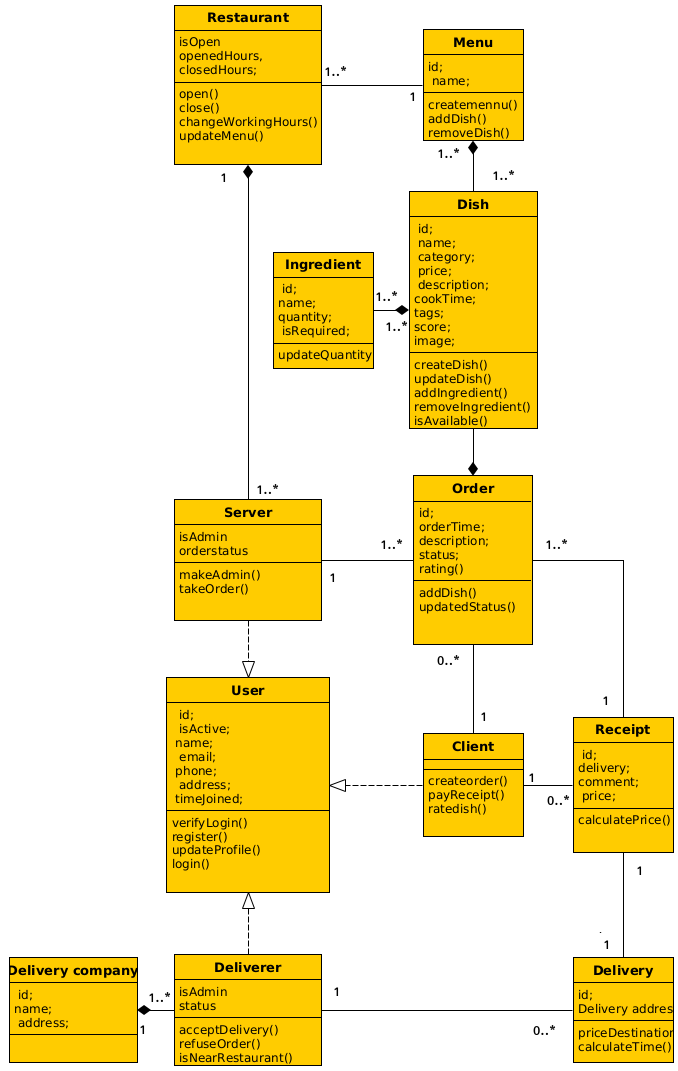
\includegraphics[width=10cm]{classdiag.png}
  				\caption{Diagramme de classes}
  				\label{fig:classdiag}
			\end{figure}
			
			La figure ci-dessus décrit les classes principales d'objets sur lesquelles repose la logique de l'application, ainsi que les relations qui existent entre eux.\\Le tableau suivant explique le schéma en figure \ref{fig:classdiag}, dans lequel les classes sont définies comme suit:
			
			\begin{table}[!h!]
  				\begin{tabular}{llll}
    					Classes & Attributs & Méthodes & Relations \\ 
    					\hline
    					Restaurant & 7 & &  \\
    					Words in the title & 2 \\
  				\end{tabular}
  				\caption{Diag}
  				\label{tab:classdiag}
			\end{table}

		\newpage
		\subsubsection{Diagrammes de cas d’utilisation}
			
			\begin{figure}[!h]
  				\center
  				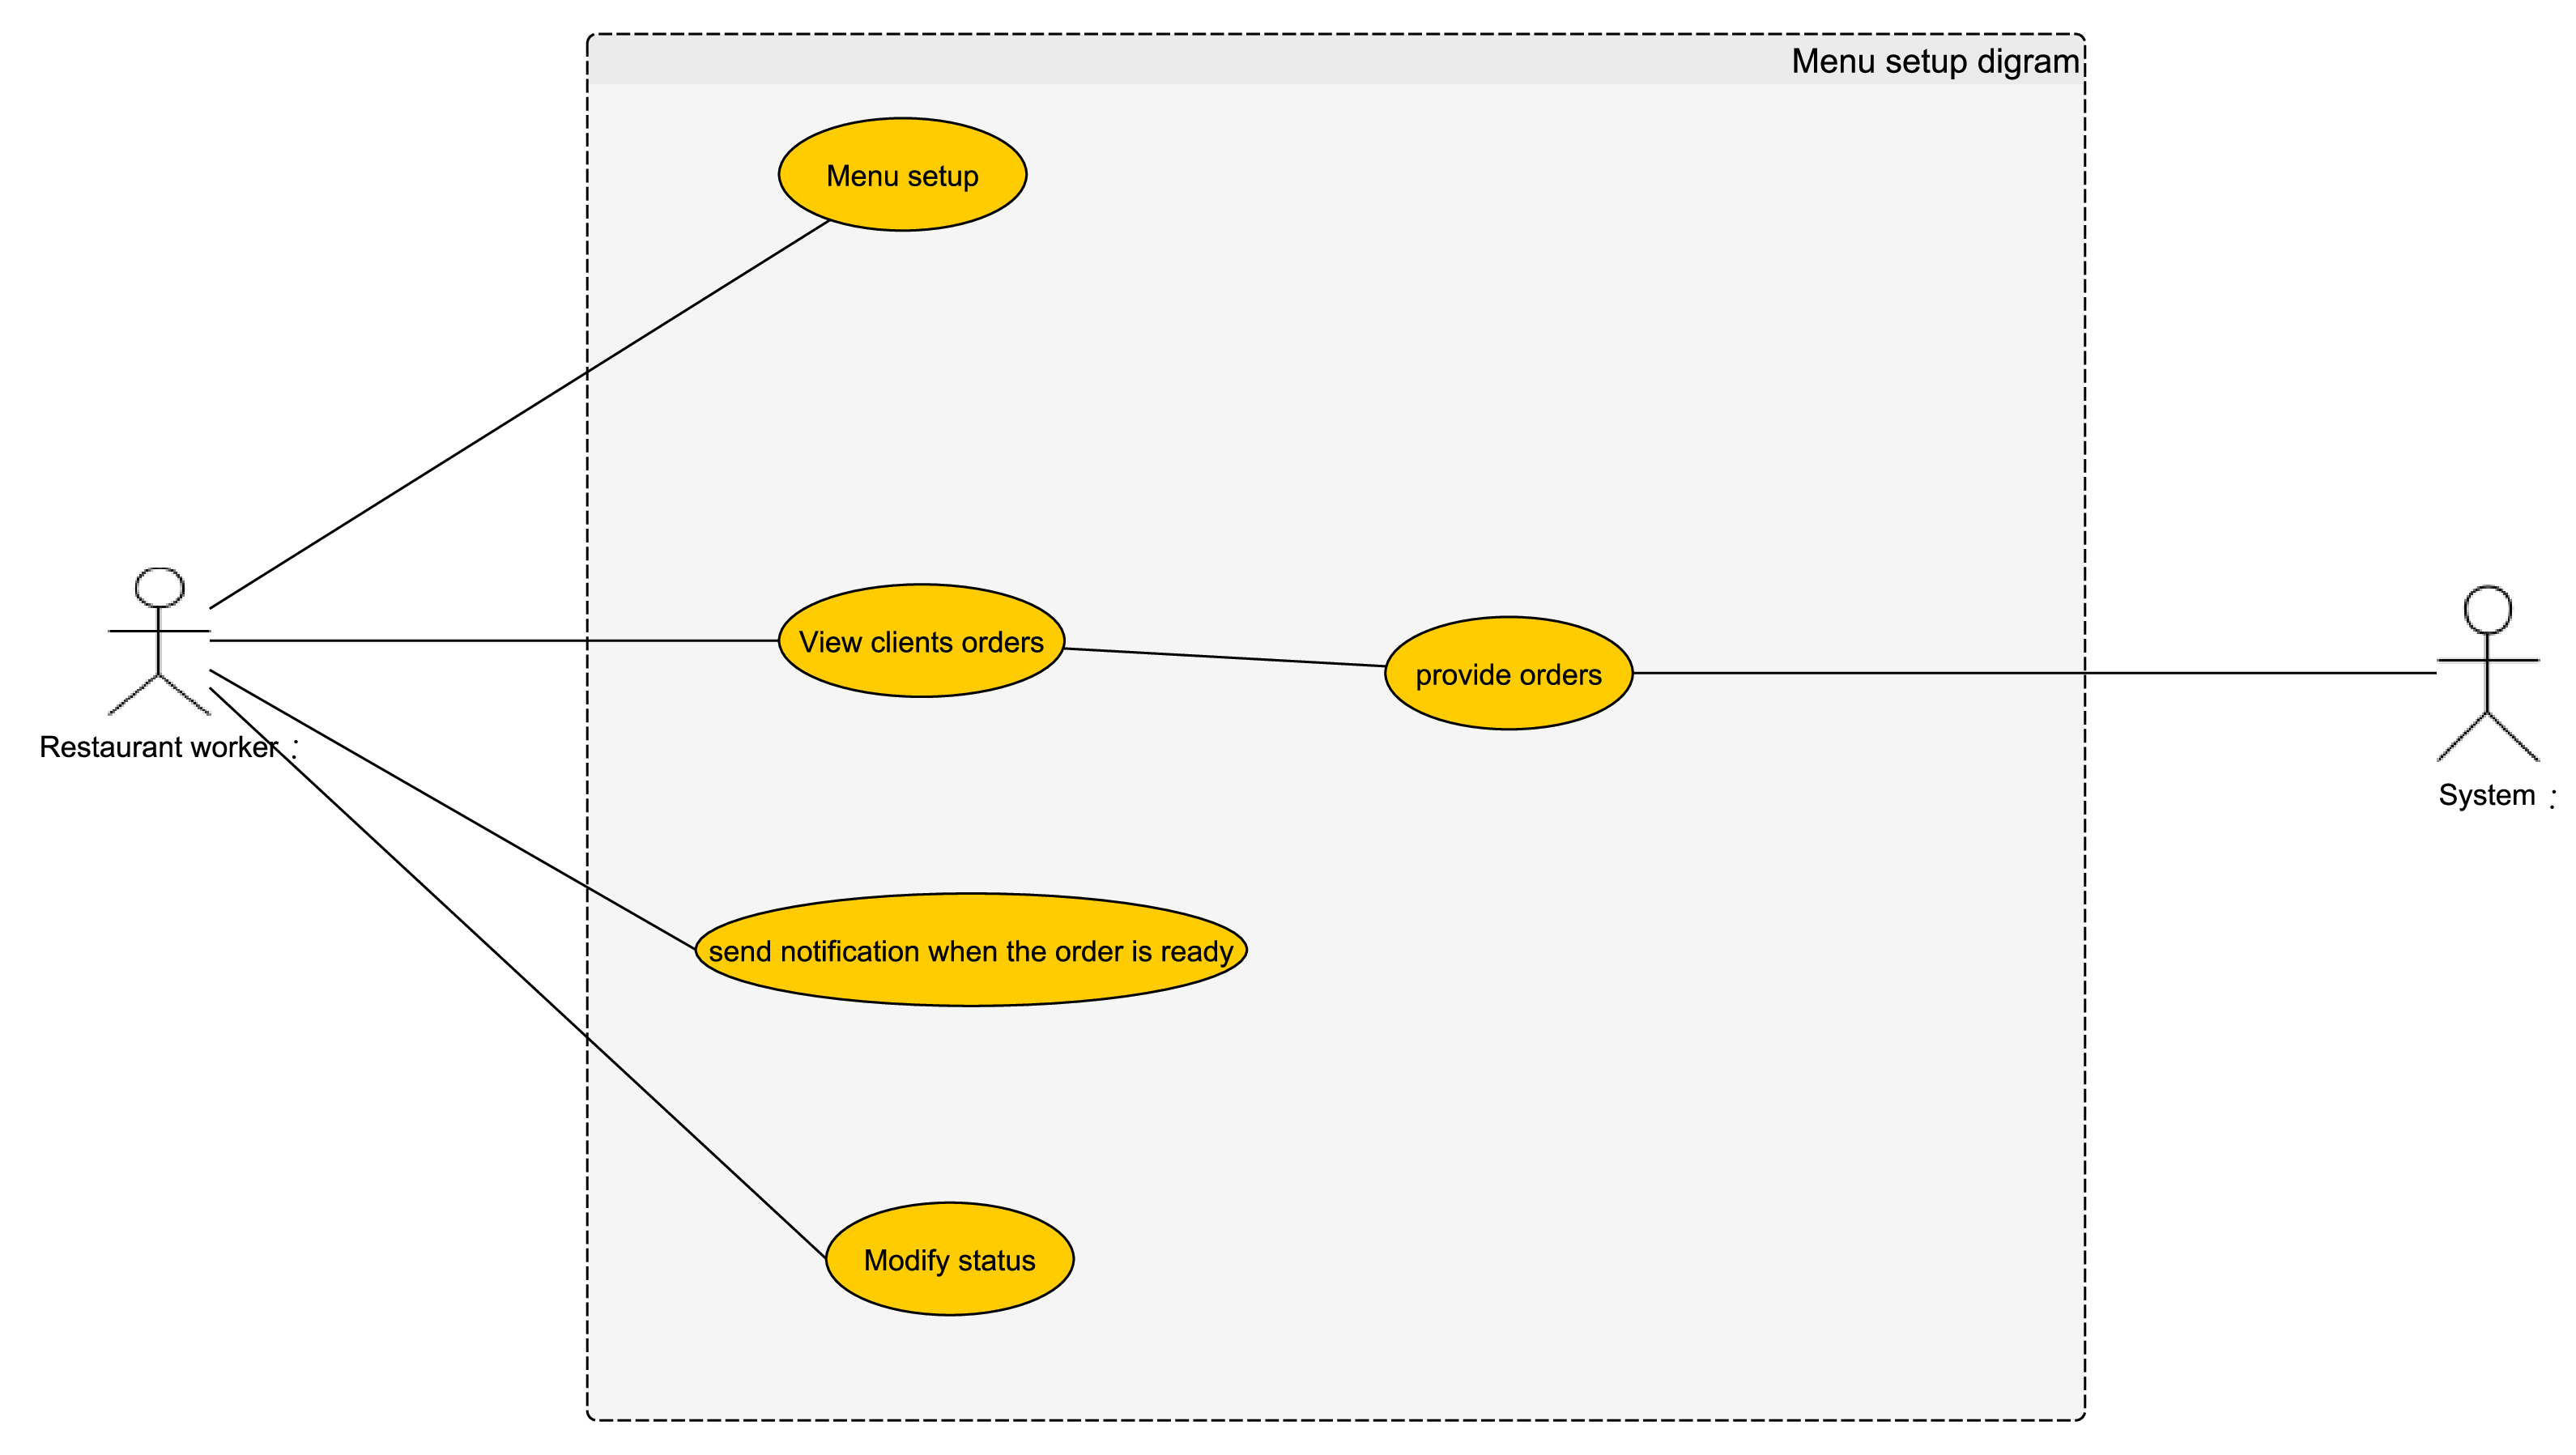
\includegraphics[width=15cm]{usecasemenu.png}
  				\caption{Diagramme de cas d'ustilisation du configuration du menu}
  				\label{fig:usecasemenu}
			\end{figure}
			
			%\newpage
			\begin{figure}[!h]
  				\center
  				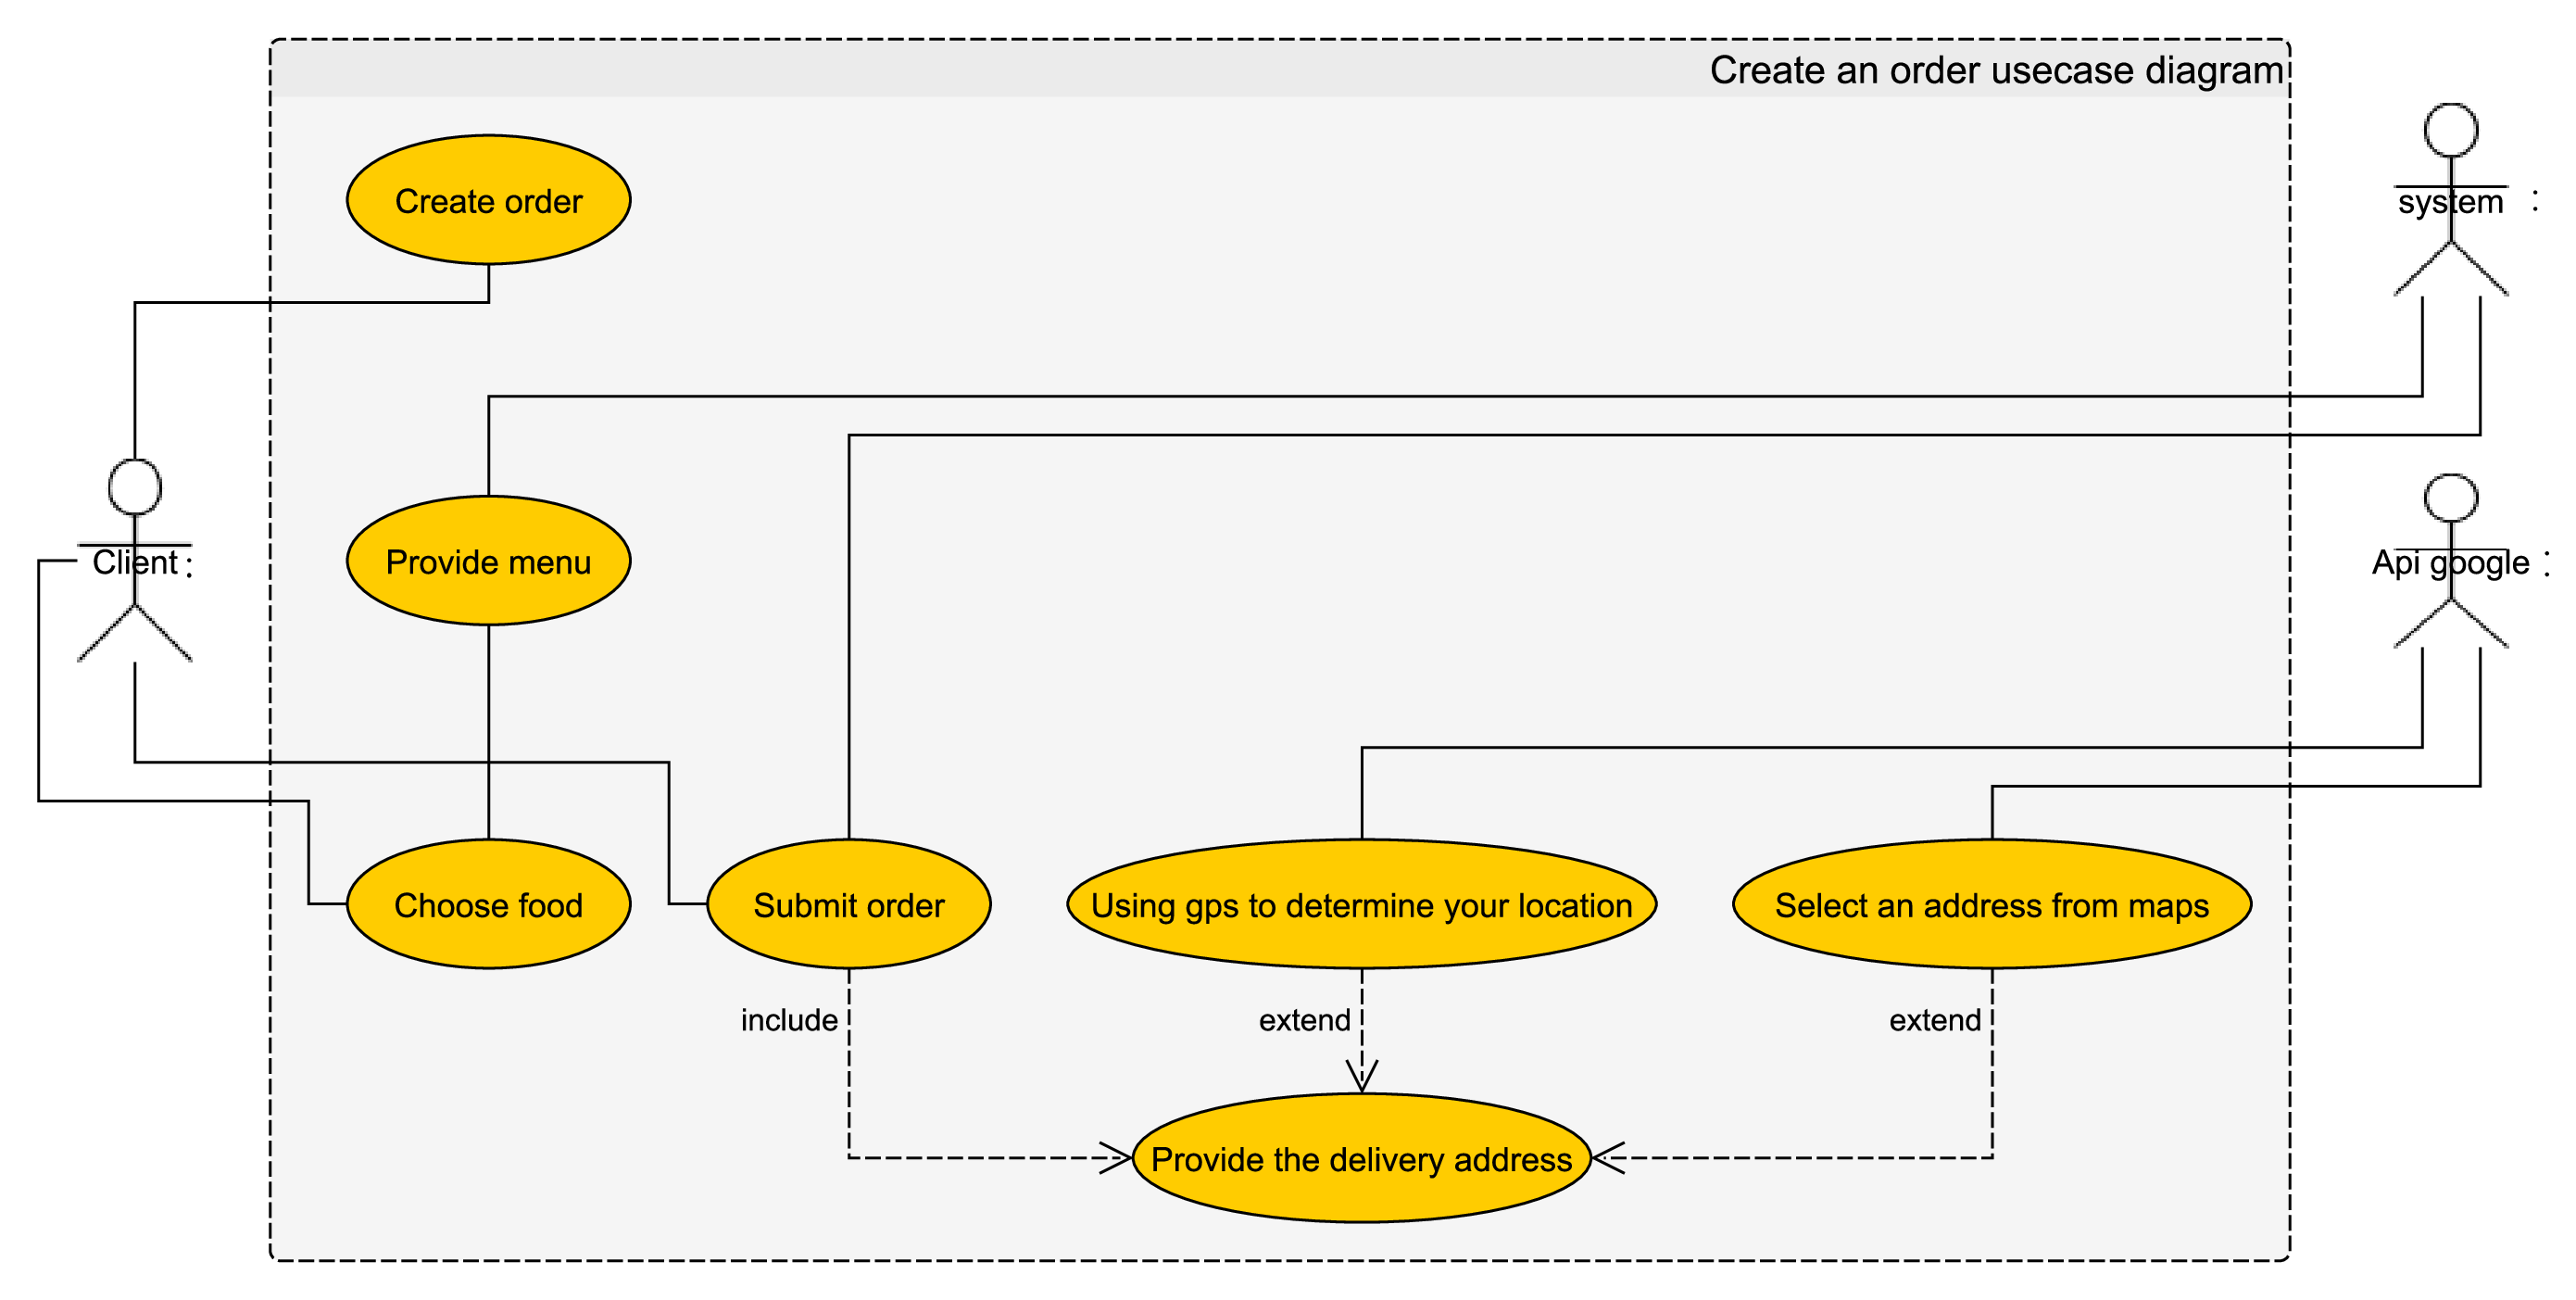
\includegraphics[width=15cm]{usecaseorder.png}
  				\caption{Diagramme de cas d'ustilisation du passation d'une commande}
  				\label{fig:usecaseorder}
			\end{figure}
			
			%\newpage
			\begin{figure}[!h]
  				\center
  				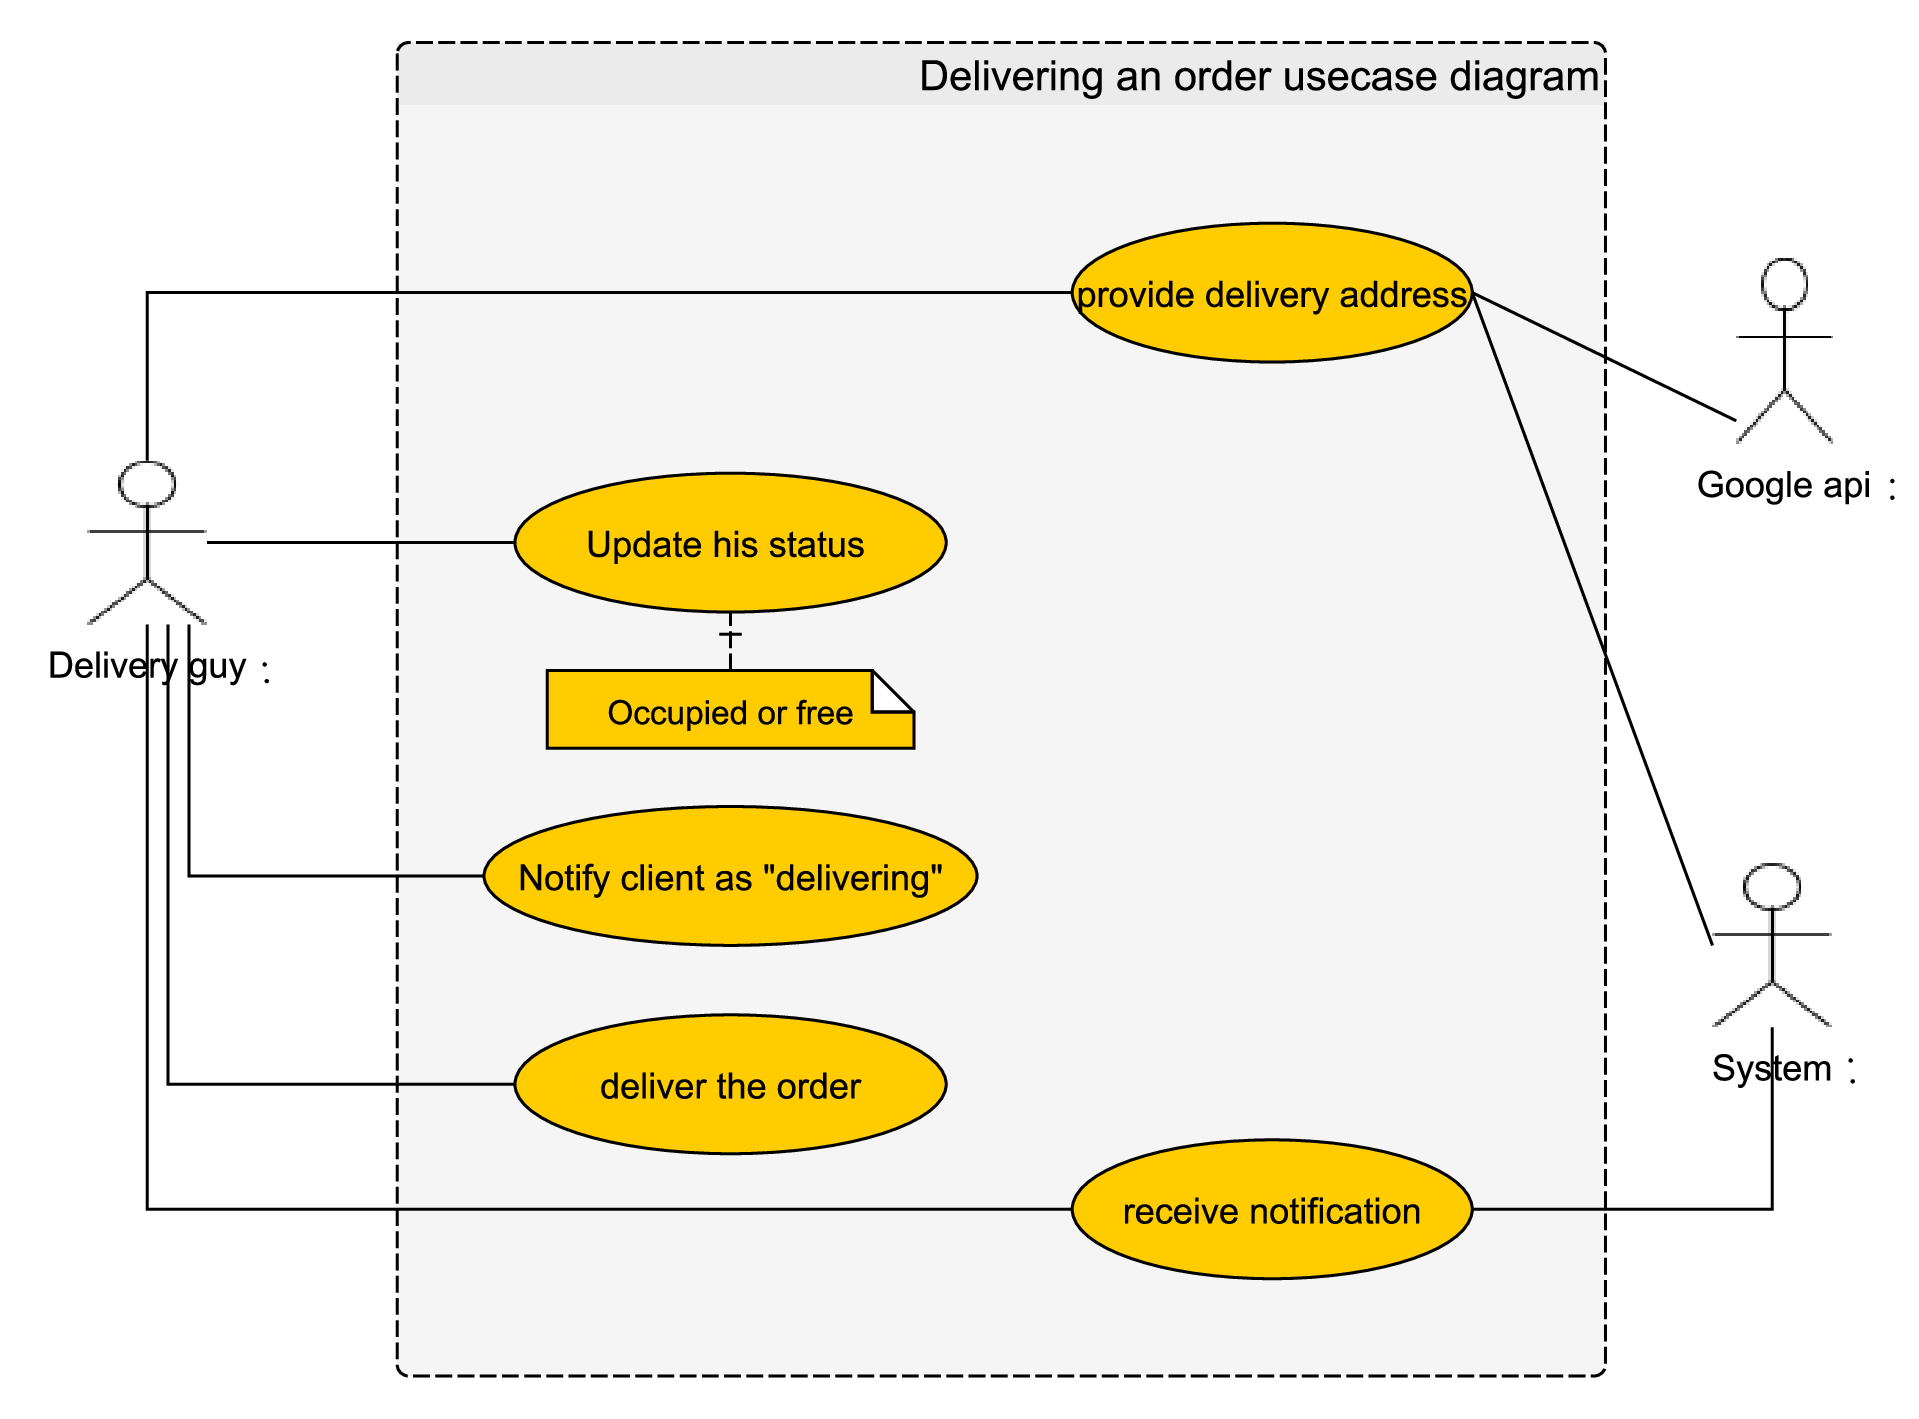
\includegraphics[width=15cm]{usecasedeliver.png}
  				\caption{Diagramme de cas d'ustilisation du livraison d'une commande}
  				\label{fig:usecasedeliver}
			\end{figure}
			\newpage
		\subsubsection{Diagrammes de séquences}
			\begin{figure}[!h]
  				\center
  				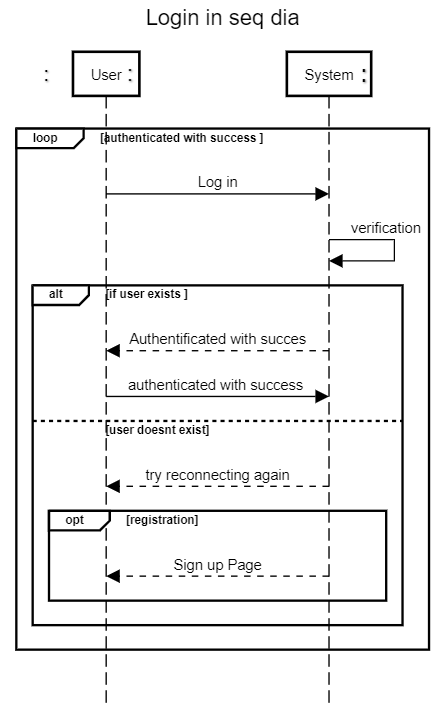
\includegraphics[width=10cm]{seqlogin.png}
  				\caption{Diagramme de séquences du authentification}
  				\label{fig:seqlogin}
			\end{figure}
			\begin{figure}[!h]
  				\center
  				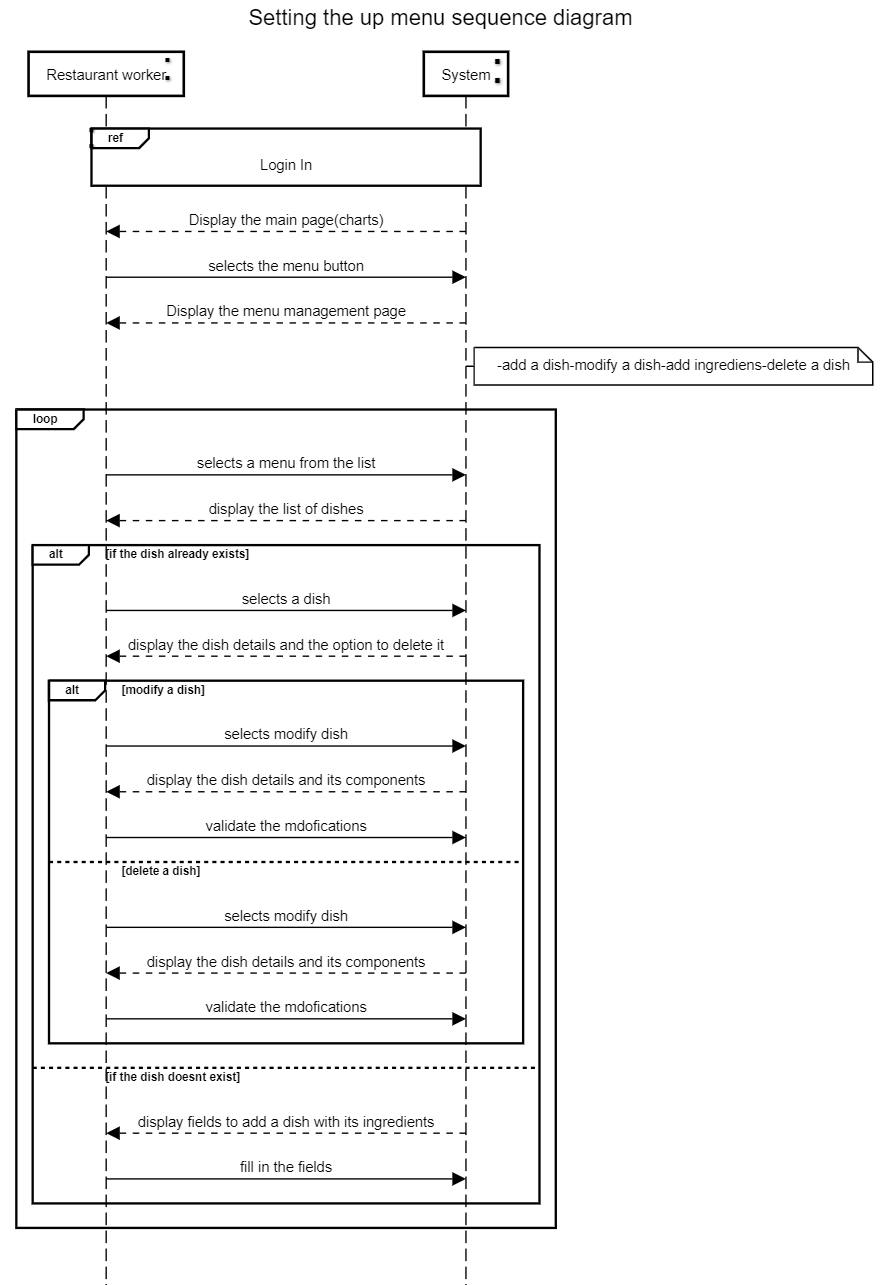
\includegraphics[width=10cm]{seqmenu.png}
  				\caption{Diagramme de séquences du configuration du menu}
  				\label{fig:seqmenu}
			\end{figure}
			\begin{figure}[!h]
  				\center
  				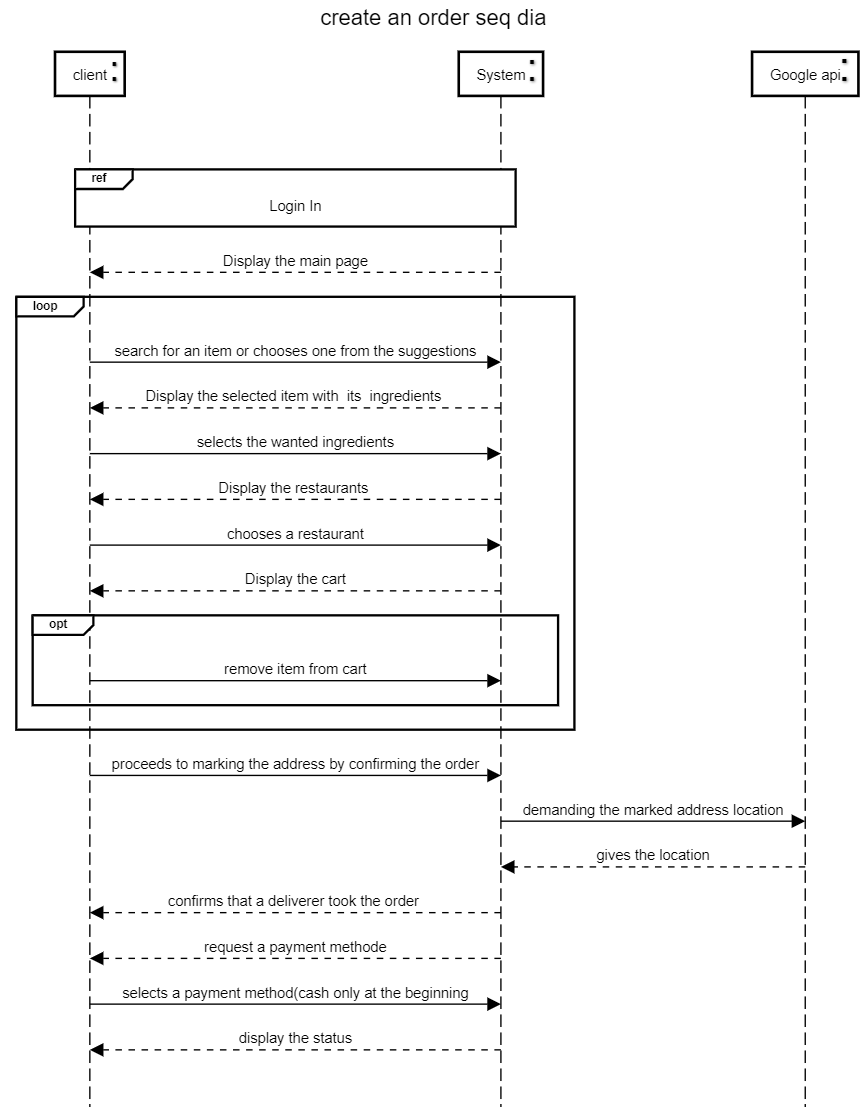
\includegraphics[width=10cm]{seqorder.png}
  				\caption{Diagramme de séquences du passation d'une commande}
  				\label{fig:seqorder}
			\end{figure}
			\begin{figure}[!h]
  				\center
  				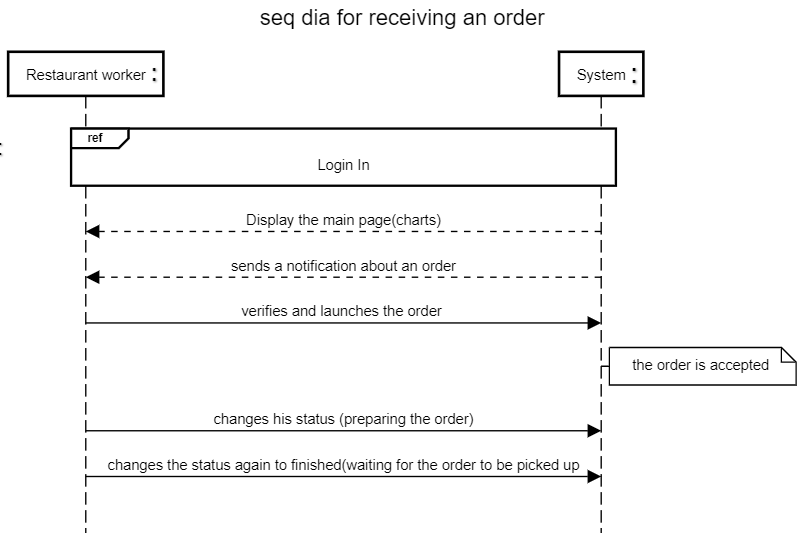
\includegraphics[width=10cm]{seqrest.png}
  				\caption{Diagramme de séquences du recepetion d'une commande}
  				\label{fig:seqrest}
			\end{figure}
			\begin{figure}[!h]
  				\center
  				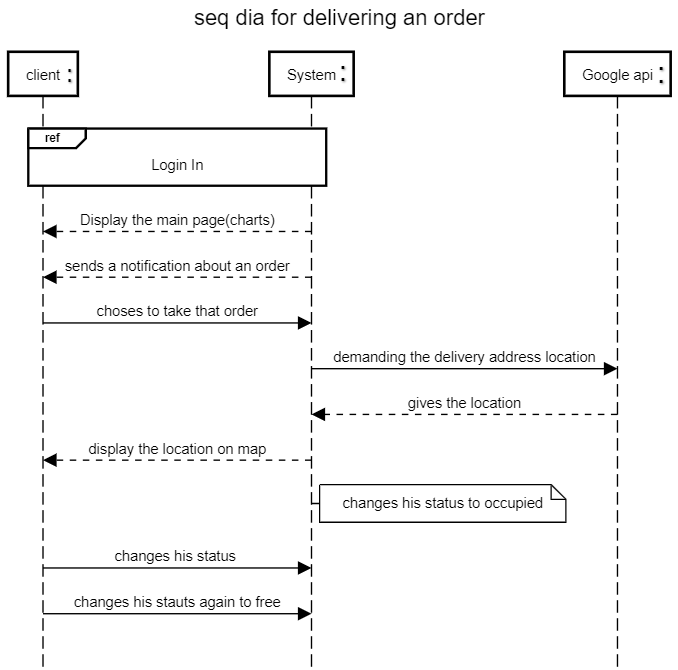
\includegraphics[width=10cm]{seqdeliver.png}
  				\caption{Diagramme de séquences du livraison d'une commande}
  				\label{fig:seqdeliver}
			\end{figure}
			
	\section{La structure du code}
		\subsection{Modéles} Nous avons représenté chaque classe du diagramme de classes (Fig. \ref{fig:classdiag}) comme des classes Dart pour les traiter comme des objets. Chacune de ces classes possède deux méthodes permettant de convertir de et vers des objets JSON  pour faciliter la communication avec la base de données.
		\subsection{Contrôleurs} Ils représentent la fonctionnalité principale de chaque action dans l'application, de la connexion à la mise à jour des commandes et tout ce qui est similaire.
		\subsection{Vues} Chaque écran qui apparaît à l'utilisateur est considéré comme une vue. Les vues contiennent plusieurs widgets en cascade.
		\subsection{Widgets} Nous avons dû créer des widgets personnalisés pour répondre à nos besoins, comme des boutons, des vues de liste, des vues de texte, etc.
		
\newpage
\chapter{Réalisation de l'application} Dans ce chapitre nous allons présenter les differentes IHMs de flux de cette application.
	\section{Startup} sign in and up
	\section{Client case} flows
	\section{Restaurant case} flows
	\section{Deliverer case} flows

\newpage
\chapter*{Conclusion}
Notre application n'est pas destinée à fonctionner avec un seul restaurant ou établissement de livraison, nous avons créé une plateforme qui regroupe tous les différents établissements pour travailler en un seul endroit.\\


Notre principal objectif en créant l'application n'était pas seulement d'apprendre à la concevoir ou d'acquérir l'expérience du développement d'une grande application mobile, mais de l'utiliser comme notre entrée dans le monde des affaires et de conquérire avec cette application le marché algérien en ligne.\\


Pour l'instant, l'application fonctionne à petite échelle, nous nous préparions à ajouter de nombreuses caractéristiques et fonctionnalités pratiques, mais en raison du peu de temps qui nous a été accordé, nous n'avons pas atteint le produit souhaité.\\


Nous allons continuer à développer cette idée et la pousser à l'extrême car nous avons remarqué que nous offrons en général une solution moins chère et plus efficace.

\addcontentsline{toc}{chapter}{Conclusion}

\newpage
\begin{thebibliography}{300}
\end{thebibliography}

\end{document}
